%%=============================================================
%%  EACS Dataset -- data description manuscript
%%  Target journal: Data in Brief (Elsevier)
%%  Template: Elsevier CAS LaTeX double-column (cas-dc.cls v2.4)
%%
%%  Compile sequence:  pdflatex -> bibtex -> pdflatex -> pdflatex
%%=============================================================
% NOTE: the "longmktitle" option is deliberately NOT used. cas-common.sty
% v2.4 routes that option through \vbox_unpack_clear:N / \vbox_set_split_to_ht:NNn,
% which are absent from the expl3 build shipped with MiKTeX 26.5. Uncomment the
% option below if you compile on Overleaf or TeX Live with a recent l3kernel.
\documentclass[a4paper,fleqn]{cas-dc}
% \documentclass[a4paper,fleqn,longmktitle]{cas-dc}

%% If a numbered (rather than author--year) citation style is
%% preferred, replace the line below with
%%   \usepackage[numbers]{natbib}
%% and set \bibliographystyle{model1-num-names}.
\usepackage[authoryear,longnamesfirst]{natbib}

%% ---- Packages -------------------------------------------------
\usepackage{graphicx}
\usepackage{amsmath,amssymb,amsthm,amsfonts}
\usepackage{booktabs}
\usepackage{array}
\usepackage{longtable}
\usepackage{enumitem}

%% ---- Column types used by the tables --------------------------
%% NB: cas-common.sty already defines L and C; only P is added here.
\newcolumntype{P}[1]{>{\raggedright\arraybackslash}p{#1}}

%% ---- Sans-serif face -------------------------------------------
%% cas-dc.cls loads the "stix" package for the serif and math faces but
%% leaves \sfdefault at "cmss". In T1 encoding that resolves to the EC
%% bitmap fonts (ecss/ecsx), which pdfTeX can only realise as Type 3
%% PK bitmaps at 600 dpi. The result is that every \sffamily run --
%% the running head, the page footer, the "Table N" / "Fig. N" labels
%% and the ARTICLE INFO / ABSTRACT headings -- is set in Computer
%% Modern Sans while the body is STIX, which reads as a font mismatch.
%% helvet loads URW Nimbus Sans as a real Type 1 family, restoring a
%% single consistent Helvetica/STIX (sans/serif) pairing.
\usepackage[scaled=0.95]{helvet}

%% ---- Captions set in the body serif ------------------------------
%% cas-common.sty builds both caption macros with \sffamily, so figure
%% and table titles come out in Nimbus Sans while the body is STIX.
%% Both macros are redefined below with \rmfamily so that every caption
%% matches the body text.
\ExplSyntaxOn
\cs_set:Npn \__make_tbl_caption:nn #1#2
  {
    \l_tbl_align_tl
    \skip_vertical:N \l_tbl_abovecap_skip
    {\parbox{\dimexpr(\l_tbl_width_dim)}
      {\rightskip=0pt\rmfamily\small
       \textbf{\color{scolor}#1}\par#2\par\vskip4pt}}
    \skip_vertical:N \l_tbl_belowcap_skip
  }

\cs_set:Npn \__make_fig_caption:nn #1#2
  {
    \l_fig_align_tl
    \skip_vertical:N \l_fig_abovecap_skip
    \setbox\cascaptionbox=\hbox
      {\rmfamily\small\textbf{\color{scolor}#1:}~#2}
    \ifdim\the\wd\cascaptionbox<\dim_use:N \l_fig_width_dim\relax
      \parbox{\l_fig_width_dim}
        {\unskip\ignorespaces\hfil\rmfamily\small
         \textbf{\color{scolor}#1:}~#2\hfil\par}
    \else
      \parbox{\l_fig_width_dim}
        {\rightskip=0pt\unskip\ignorespaces\rmfamily
         \small\textbf{\color{scolor}#1:}~#2\par}
    \fi
    \skip_vertical:N \l_fig_belowcap_skip
  }
\ExplSyntaxOff

%% ---- Page header and footer in the body serif -------------------
%% CAS sets the running head and the footer in \sffamily. They are
%% redefined here in \rmfamily so that no part of the page furniture
%% departs from the STIX body face.
\ExplSyntaxOn
\cs_set:Npn \__cas_head:
  {
    \parbox{\textwidth}
      {\rmfamily\small\centering \__short_title:}
  }

\cs_set:Npn \__cas_foot:
  {
    \parbox[t]{\textwidth}
      {
        \rule{\textwidth}{.2pt}\\
        \rmfamily\small
        \hfill Page~\thepage {}~of~ \lastpage
      }
  }

\cs_set:Npn \__first_foot:
  {
    \parbox[t]{\textwidth}
      {
        \rule{\textwidth}{.2pt}\\
        \rmfamily\small
        \hfill Page~\thepage {} ~of~ \lastpage
      }
  }

%% The CAS preprint footer reads "Short Author: Preprint submitted to
%% Elsevier". The second half was removed earlier as requested, which
%% would leave the author name sitting after a colon with nothing
%% following it. The running head already carries the short title and
%% the author is named on the title page, so the footer keeps only the
%% page number.
\cs_set:Npn \__first_footerline: { }
\ExplSyntaxOff

%% cas-common.sty runs \ps@cas at load time, and \ps@cas copies the
%% four header/footer macros into \@oddhead, \@evenhead, \@oddfoot and
%% \@evenfoot with \cs_set_eq:NN. Re-running it here makes those slots
%% pick up the redefinitions above. The command name contains "@", so
%% it needs \makeatletter.
\makeatletter
\ps@cas
\makeatother

%% ---- Float placement ------------------------------------------
%% The manuscript carries five figures and three tables, three of
%% which span both columns. LaTeX's default float thresholds are too
%% strict for that mix and push full-width floats onto float-only
%% pages, leaving large gaps; relaxing them keeps text and floats on
%% the same page.
\renewcommand{\topfraction}{0.85}
\renewcommand{\dbltopfraction}{0.85}
\renewcommand{\bottomfraction}{0.6}
\renewcommand{\textfraction}{0.08}
\renewcommand{\floatpagefraction}{0.6}
\renewcommand{\dblfloatpagefraction}{0.6}
\setlength{\textfloatsep}{14pt plus 3pt minus 4pt}
\setlength{\dbltextfloatsep}{16pt plus 4pt minus 6pt}
\setlength{\dblfloatsep}{10pt plus 2pt minus 3pt}
\setcounter{topnumber}{3}
\setcounter{dbltopnumber}{3}
\setcounter{totalnumber}{4}

%% Note on bibliography spacing: \bibsep cannot be tightened from
%% here. cas-common.sty executes \bibsep=0pt unconditionally, so the
%% list is already set solid and any \setlength issued in this
%% preamble is discarded.

%% ---- Caption labels --------------------------------------------
%% cas-common.sty defaults to "Figure N"; Elsevier house style --
%% and the in-text references used below -- is "Fig. N".
\renewcommand{\figurename}{Fig.}
\renewcommand{\tablename}{Table}

%% ---- Tolerate tight double-column measure --------------------
%% Long typewriter tokens (file names) and long capitalised words
%% otherwise produce a scattering of small overfull boxes.
\setlength{\emergencystretch}{2em}
\hyphenation{da-ta-base men-de-ley Na-tion-al-School-In-tra ran-dom-ised
  ran-dom-ised ran-dom-i-sa-tion an-onym-i-sa-tion}

%% ---- Dataset macros -------------------------------------------
\newcommand{\datasetname}{EACS Dataset}
\newcommand{\datasetdoi}{10.17632/mvzdksjzvb.1}
\newcommand{\datasetdoiurl}{\href{https://doi.org/10.17632/mvzdksjzvb.1}{10.17632/mvzdksjzvb.1}}
\newcommand{\dataseturl}{\url{https://data.mendeley.com/datasets/mvzdksjzvb/1}}

\begin{document}
\let\WriteBookmarks\relax
\def\floatpagepagefraction{1}
\def\textpagefraction{.001}

% ---- Running head ----------------------------------------------
\shorttitle{EACS Dataset: real-world academic admit cards}
\shortauthors{Ashadzzaman}

% ---- Title ------------------------------------------------------
\title[mode=title]{EACS Dataset: 4,407 real-world Bangladeshi admit card
images with field-level ground truth for OCR and document understanding}

% The CAS \tnotemark/\tnotetext pair attaches a "\*"-style footnote
% marker to the title. It is left out so the title carries no symbol.
% The repository and DOI it pointed at are already given in Table 1
% and in the Data availability statement.
% \tnotemark[1]
% \tnotetext[1]{The dataset described in this article is deposited on
% Mendeley Data at \dataseturl{} (doi: \datasetdoiurl).}

% ---- Author block ------------------------------------------------
\author[1]{Baizid MD Ashadzzaman}[orcid=0009-0008-4137-5905]

\cormark[1]
\ead{baizid.md.ashadzzaman@gmail.com}
\ead[url]{https://orcid.org/0009-0008-4137-5905}

\credit{Conceptualization, Methodology, Software, Data curation, Validation,
Investigation, Visualization, Writing: original draft, Writing: review and editing}

\affiliation[1]{organization={Department of Computer Science and Engineering,
International Islamic University Chittagong},
            city={Chattogram},
            postcode={4221},
            country={Bangladesh}}

\cortext[1]{Corresponding author}

% ---- Abstract ------------------------------------------------------
\begin{abstract}
Educational institutions in South Asia issue large volumes of machine-printed
examination admit cards, yet no openly available corpus exists for research on
optical character recognition (OCR) or automated verification of such documents.
This data paper presents the EACS (Exam Admit Card) Dataset: 4{,}407 admit card
images collected between 2022 and 2025 from the NationalSchoolIntra enterprise
resource planning platform operated by Al Quran Academy, Chattogram, Bangladesh.
Each record is a standardised $800 \times 460$ pixel JPEG rendering of one card
and carries nine textual fields (student name, father's name, mother's name,
institutional student identifier, examination roll number, class, session, group
and semester) together with the list of registered subjects and the scheduled
examination date. A companion metadata file supplies a verified ground-truth
transcription for every field of every card, so that recognition error can be
measured at character, word and field level. The images were exported from the
live production system rather than generated synthetically, and consequently
retain the typographic, alignment and print-quality variation that synthetic
corpora typically omit, a property that materially affects measured OCR
accuracy. Student photographs, contact details and signatures were removed, and
all personal names and identifiers were systematically randomised while
preserving their structural and linguistic characteristics, allowing the corpus
to be distributed openly. The dataset is released on Mendeley Data (version 1,
doi: \datasetdoi). Intended applications include OCR benchmarking, document
layout analysis, key-information extraction from administrative documents, and
the development of tamper-detection mechanisms for academic credentials.
\end{abstract}

% ---- Highlights ---------------------------------------------------
% The CAS "highlights" environment reserves a separate unnumbered page
% for the bullet list. It is left out here so that the manuscript
% opens directly on the title page. Restore the block below (or paste
% the five bullets into Elsevier's submission system) if the target
% journal asks for Highlights.
% \begin{highlights}
% \item 4{,}407 real admit card images exported from a live school ERP system.
% \item Nine annotated textual fields per card with verified ground truth.
% \item Genuine print, alignment and font variation across four annual sessions.
% \item All personal identifiers removed or randomised prior to release.
% \item Deposited on Mendeley Data under a citable DOI.
% \end{highlights}

% ---- Keywords -----------------------------------------------------
\begin{keywords}
Optical character recognition \sep Document image analysis \sep Admit card
dataset \sep Document verification \sep Key information extraction \sep
Educational data \sep Bangladeshi academic documents
\end{keywords}

\maketitle

%=================================================================
\section{Introduction}
%=================================================================

Admissions and examination administration in large secondary schools is a
high-volume, highly repetitive clerical process. At the institution from which
the present corpus was drawn, examination admit cards are generated once per
student per session (several thousand documents per examination cycle) and
the resulting registers are transcribed into downstream information systems
either by hand or through ad hoc optical character recognition (OCR) pipelines.
Both routes are error-prone. Manual transcription introduces omissions and
character confusions that are difficult to audit, while general-purpose OCR
engines degrade noticeably on the typographic register of institutional
forms: serif typefaces, inconsistent baseline alignment, mixed Latin and
Arabic-derived numerals, and condensed tabular layouts \citep{smith2007,
reuel2019}.

Reproducing that degradation in a laboratory is not straightforward. The
benchmarks most often used to compare OCR systems are built from born-digital
documents or from natural-scene photographs \citep{jaderberg2014}, both of
which differ substantially from a laser- or inkjet-printed administrative form
emitted by an enterprise resource planning (ERP) system. Consequently, published
accuracy figures transfer poorly to the documents that schools and universities
actually process, and researchers who need realistic error estimates have no
standard corpus against which to calibrate them.

This gap is wider for South Asian academic documents than the general
literature suggests. The large public document-analysis corpora, for example
PubLayNet \citep{zhong2019} and TableBank \citep{li2019}, consist of
scientific articles and are annotated at the level of layout regions and table
structure, not at the level of individual administrative fields. Nothing in
that collection is representative of a school examination register printed in
English for a Bangladeshi institution, with its particular field order, class
and group nomenclature, and subject coding scheme.

The EACS Dataset was assembled to close that gap. It provides (i) a
representative collection of real, operationally generated admit card images;
(ii) field-level ground-truth transcriptions aligned one-to-one with those
images; and (iii) the anonymisation required for open redistribution. The
present article describes the corpus in the format expected of a data
descriptor \citep{elsevier2024}, and states explicitly the limitations that
users should account for when drawing conclusions from it.

%=================================================================
\section{Related work}
%=================================================================

\subsection{Optical character recognition and its evaluation}

Tesseract \citep{smith2007} remains the most widely deployed open-source OCR
engine and is the default baseline in comparative evaluations;
\citet{reuel2019} benchmarked it against a range of contemporary alternatives
and documented large variation in accuracy across engines, scripts and
acquisition conditions. That variation is the reason benchmark corpora matter:
an accuracy figure is meaningful only relative to the document population it
was measured on. The present corpus is offered as one additional, explicitly
described population (operational, low-complexity, South Asian academic
forms) against which such comparisons can be run.

\subsection{Sequence models and the role of representative training data}

Modern recognisers are broadly sequence-to-sequence models, historically
derived from bidirectional long short-term memory architectures
\citep{graves2005}, which replaced the hand-engineered character classifiers
of earlier systems with learned representations. Learning those
representations is data-hungry, and the field has therefore leaned heavily on
synthetic corpora, most influentially SynthText \citep{ba2016}, which renders
arbitrary text into arbitrary backgrounds to achieve large scale. Synthetic
generation solves the volume problem but introduces a domain gap: synthetic
samples are smooth, uniformly contrasted and geometrically regular, whereas
scanned or printed administrative documents contain speckle, toner dropout,
baseline drift and inconsistent kerning. A model tuned predominantly on
synthetic data can score well on synthetic held-out sets and noticeably worse
on production documents. Corpora such as EACS are therefore needed as
evaluation, and optionally fine-tuning, material.

\subsection{Document layout analysis}

Layout analysis, which partitions a page into semantic regions, has been
served by several large annotated corpora. PubLayNet \citep{zhong2019}
segments journal pages into text, title, list, table and figure regions;
TableBank \citep{li2019} provides both detection and structure recognition for
tables. Both derive from machine-readable academic articles. EACS
complements them with a form-like document type: a single record per image,
a fixed field inventory, and a stable reading order, which is the regime that
key-information-extraction pipelines for administrative automation must handle.

\subsection{Document tampering and credential verification}

The same admit cards that are useful for OCR research are attractive targets
for forgery, because a convincing credential can be produced by editing text
within an otherwise genuine card. Statistical tests operating in the
transformed or compressed domain have long been used to detect such
manipulation \citep{fridrich2004,goljan2012}. The forensic value of those
tests depends on having authentic reference material drawn from the same
issuing pipeline as the suspect document, which is precisely what an openly
released corpus of unedited operational cards provides. Broader surveys of
credential and phishing abuse \citep{almakhour2018} underline the practical
motivation for automated verification of academic documents.

%=================================================================
\section{Data source and acquisition}
%=================================================================

Fig.~\ref{fig:pipeline} summarises how records moved from the institution's
production system to the released corpus. Each stage is described in the
subsections that follow. The two controls that either remove records or gate
the release, the image-to-database check and the governance review, are drawn
explicitly so that the composition of the final 4,407 records can be
accounted for.

\begin{figure}[width=\linewidth,cols=1,pos=htbp]
\centering
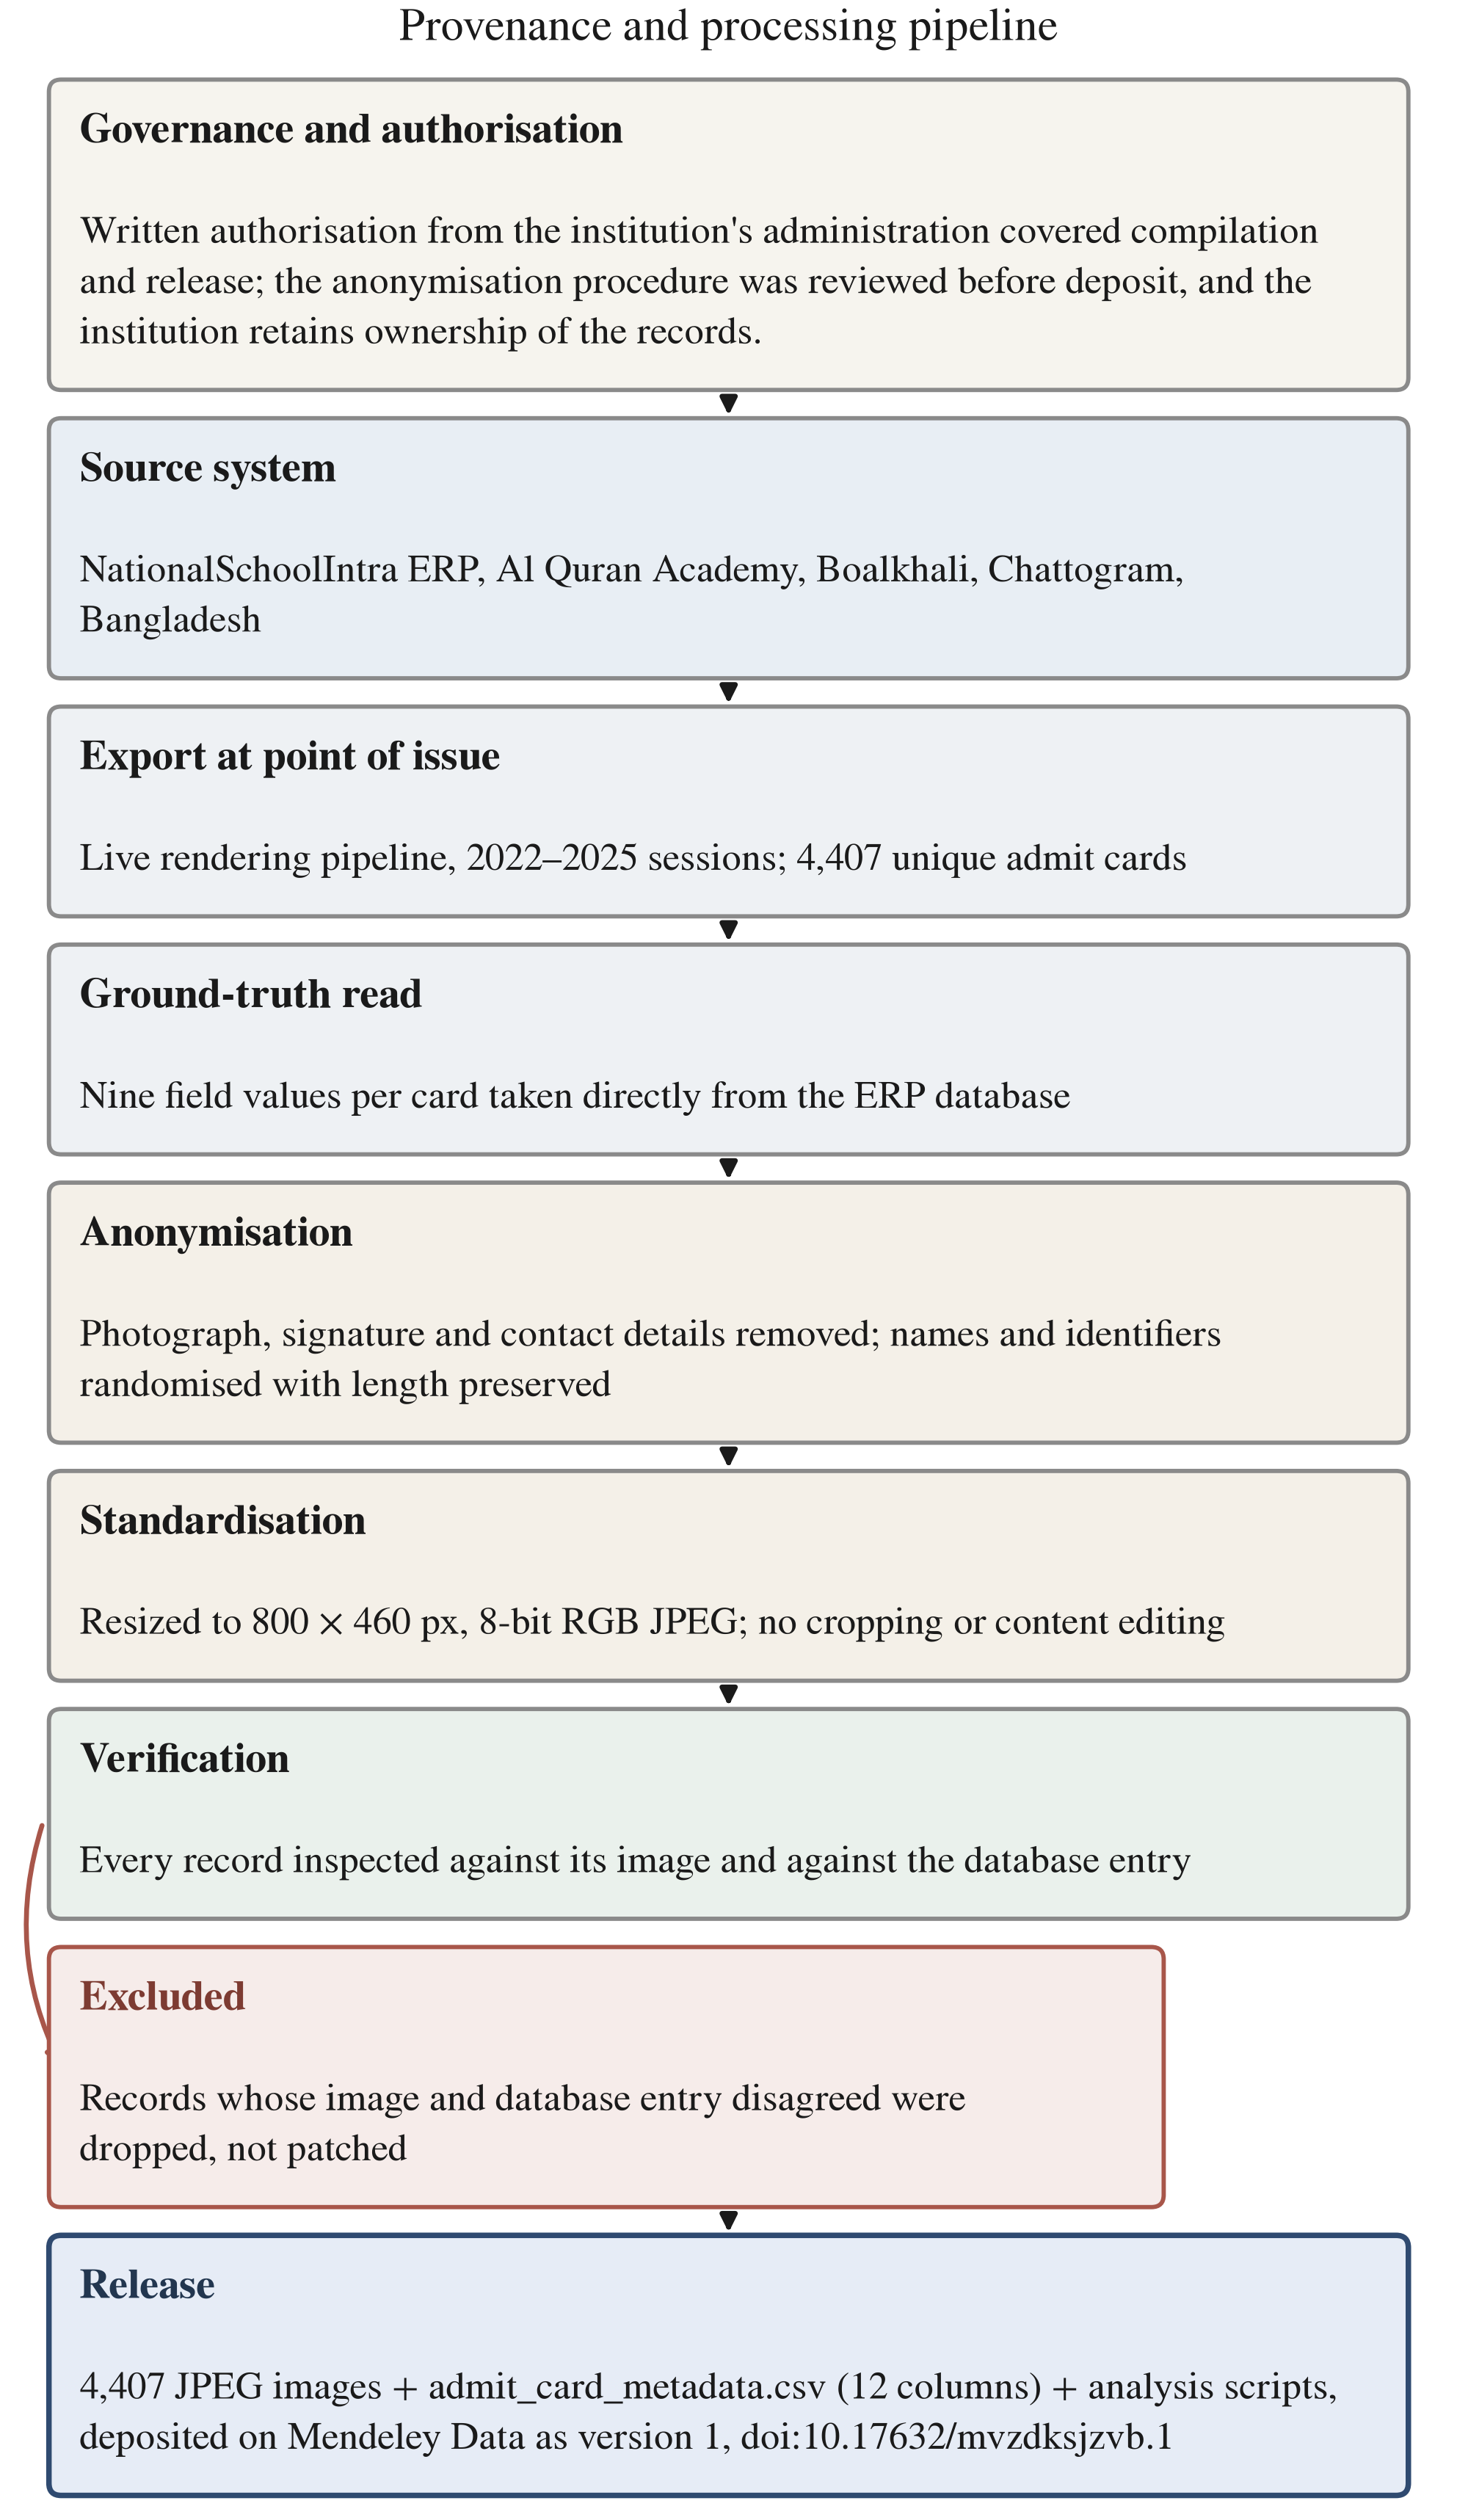
\includegraphics[width=\linewidth]{figures/fig6_pipeline.png}
\caption{Provenance and processing pipeline. Records were exported from the live
NationalSchoolIntra ERP rendering pipeline at the moment of issue, read for ground
truth from the same database, anonymised, standardised to a common canvas, and
then checked against both image and database before release. Records whose image
and database entry disagreed were excluded rather than patched.}
\label{fig:pipeline}
\end{figure}

\subsection{Origin}

All records originate from the NationalSchoolIntra ERP platform
\citep{nationalschoolintra}, the production system used by Al Quran Academy,
Boalkhali, Chattogram, Bangladesh, for student enrolment, examination
scheduling and card generation. Cards were exported directly from the live
rendering pipeline at the moment of issue, between the 2022 and 2025 academic
sessions, yielding 4{,}407 unique records. Because the corpus is drawn from a
running system rather than reconstructed for research, it inherits that
system's template revisions, misaligned fields and print artefacts.

\subsection{Authorisation}

Compilation and release were carried out with the written authorisation of the
institution's administration, which retains ownership of the underlying
records and reviewed the anonymisation procedure described in
Section~\ref{sec:ethics} before release.

\subsection{Standardisation}

To keep the corpus homogeneous and storage-efficient, every exported record was
resized to a fixed $800 \times 460$ pixel canvas and encoded as JPEG. Card
templates share a common geometry, so this operation preserves the relative
position and scale of all text regions; no cropping, rotation correction or
content editing was applied. Field text was not redrawn or typeset by the
authors; the images are the artefacts the system actually produced.

\subsection{Analytical tooling}

Summary statistics and all figures in this article were produced with the
Python scientific stack \citep{mckinney2010,virtanen2020} and Matplotlib
\citep{hunter2007}. The analysis scripts are distributed with the dataset so
that every reported quantity can be regenerated from the released files.

%=================================================================
\section{Dataset description}
\label{sec:description}
%=================================================================

Table~\ref{tab:specs} summarises the corpus. Table~\ref{tab:schema} gives the
complete field inventory, and
Figs.~\ref{fig:layout}--\ref{fig:namelen} characterise its composition.

\begin{table*}[width=\FullWidth,cols=2,pos=htbp]
\rmfamily
\caption{Specifications of the EACS Dataset.}
\label{tab:specs}
\begin{tabular}{@{}P{0.225\textwidth}P{0.715\textwidth}@{}}
\toprule
\textbf{Item} & \textbf{Description} \\
\midrule
Name          & EACS Dataset (Exam Admit Card Dataset) \\
Subject area  & Document image analysis, optical character recognition and
                educational document verification \\
Type of data  & Document images (JPEG) and tabular ground truth (CSV) \\
Data format   & 8-bit RGB JPEG, $800 \times 460$ pixels; UTF-8 CSV \\
How acquired  & Exported from the production rendering pipeline of the
                NationalSchoolIntra ERP system at Al Quran Academy, Boalkhali,
                Chattogram, Bangladesh \\
Collection    & 4{,}407 admit cards issued across the 2022--2025 academic
                sessions \\
Ground truth  & Field-level transcription for every card, verified against the
                issuing system \\
Anonymisation & Photographs, contact details and signatures removed; all names
                and identifiers randomised with structure and length preserved \\
Source        & Al Quran Academy, Boalkhali, Chattogram, Bangladesh \\
Repository    & Mendeley Data, version 1, doi: \datasetdoiurl \\
\bottomrule
\end{tabular}
\end{table*}

\subsection{Document layout}

Fig.~\ref{fig:layout} shows a representative card and the field regions
identified on it. The template divides into a branded header carrying the
institution name and examination title, an identification block with the
student's name, guardian names and institutional identifier, an examination
block with roll number, class, session, group and semester, and a lower band
listing the registered subjects with their numeric codes.

\begin{figure*}[width=\FullWidth,cols=1,pos=htbp]
\centering
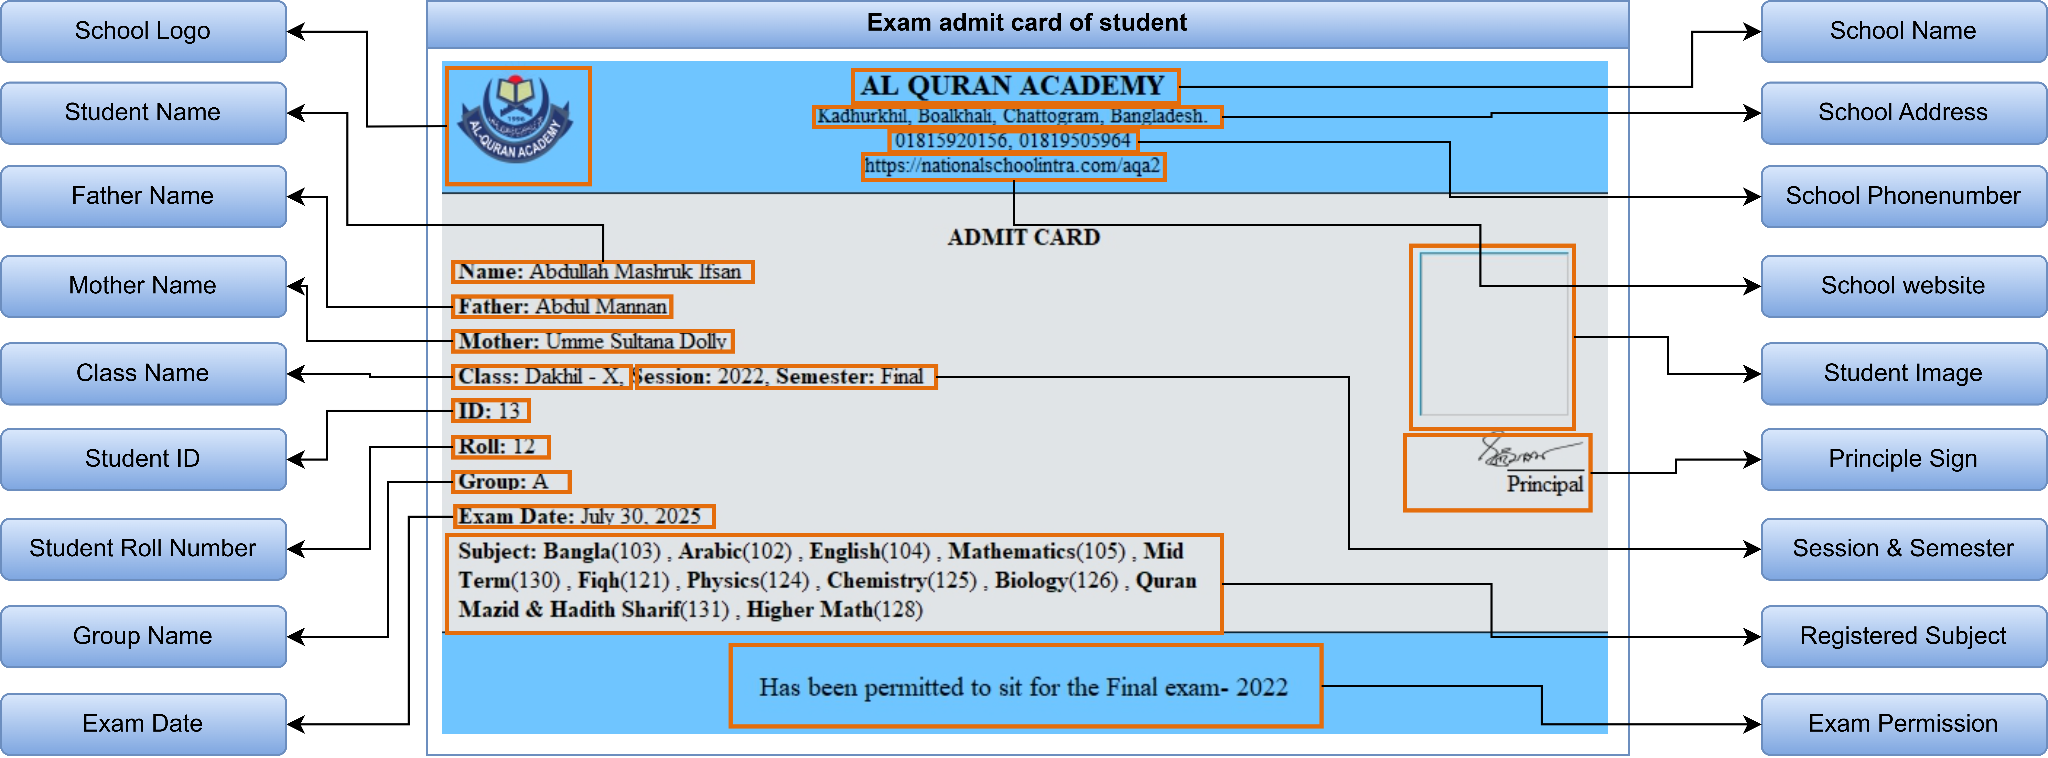
\includegraphics[width=\linewidth]{figures/fig1_document_layout.png}
\caption{Anatomy of an EACS admit card. The upper band carries institutional
branding and the examination title; the central block contains the nine
transcribed fields; the lower band lists registered subjects and their numeric
codes. Field geometry is fixed by the card template, so the regions shown here
are stable across the whole corpus.}
\label{fig:layout}
\end{figure*}

\subsection{Field inventory and metadata schema}

Nine textual fields are transcribed for every card: \texttt{student\_name},
\texttt{father\_name}, \texttt{mother\_name}, \texttt{student\_id},
\texttt{roll}, \texttt{class}, \texttt{session}, \texttt{group} and
\texttt{semester}. These are the fields that vary per record and that an OCR
pipeline must recover. Three further columns (the image filename, the
scheduled examination date and the list of registered subjects) carry
record-level rather than per-field information and support joining and
date-aware analysis. Table~\ref{tab:schema} lists all twelve columns of the
companion CSV.

The distinction matters for evaluation design. Because the template fixes field
positions, a system may be scored in three ways: recognition accuracy on the
character stream, word-level accuracy after segmentation, or field-level
exact-match accuracy once the recognised string is assigned to a region and
compared with the reference. The released ground truth supports all three
because transcription is stored per field rather than as a single flattened
page string (Section~\ref{sec:annotation}).

\begin{table*}[width=\FullWidth,cols=4,pos=htbp]
\rmfamily
\caption{The twelve columns of the accompanying metadata file
(\texttt{admit\_card\_metadata.csv}). One row per admit card image, keyed on
\texttt{admit\_card\_image}. Nine columns hold the transcribed fields; the
remaining three are record-level metadata.}
\label{tab:schema}
\footnotesize
\begin{tabular}{@{}P{0.165\textwidth}P{0.075\textwidth}P{0.44\textwidth}P{0.235\textwidth}@{}}
\toprule
\textbf{Column} & \textbf{Type} & \textbf{Description} & \textbf{Example} \\
\midrule
\texttt{admit\_card\_image}
  & string & Filename of the card image; primary key.
  & \texttt{14-699-1-1-1-1.jpg} \\
\texttt{student\_id}
  & integer & Institutional identifier (randomised).
  & \texttt{14} \\
\texttt{student\_name}
  & string & Student name as printed (randomised).
  & Abid Anwar \\
\texttt{father\_name}
  & string & Father's name as printed (randomised).
  & Mohammed Nurul Anwar \\
\texttt{mother\_name}
  & string & Mother's name as printed (randomised).
  & Mosammat Sabekun Nahar Shafu \\
\texttt{roll}
  & integer & Examination roll number.
  & \texttt{13} \\
\texttt{class}
  & string & Grade level and examination stage.
  & Dakhil - X \\
\texttt{session}
  & integer & Session year of issue.
  & \texttt{2022} \\
\texttt{semester}
  & string & Examination stage.
  & Final \\
\texttt{group}
  & string & Academic stream or group (e.g.\ Science/Arts).
  & A \\
\texttt{exam\_date}
  & date & Scheduled examination date, as printed.
  & 30-Jul-25 \\
\texttt{subjects}
  & string & Registered subjects with their codes, comma-separated.
  & Bangla (103), Arabic (102), English (104), Mathematics (105), \ldots \\
\bottomrule
\end{tabular}
\end{table*}

\subsection{Composition of the corpus}

Fig.~\ref{fig:classsession} gives the number of cards per class and session.
The corpus is not class-balanced: senior classes contribute more records than
junior ones, and volume grows across sessions, reflecting cohort growth at the
institution. Users who train models on this corpus should sample or reweight
accordingly rather than assuming a uniform prior over classes.

\begin{figure}[width=\linewidth,cols=1,pos=htbp]
\centering
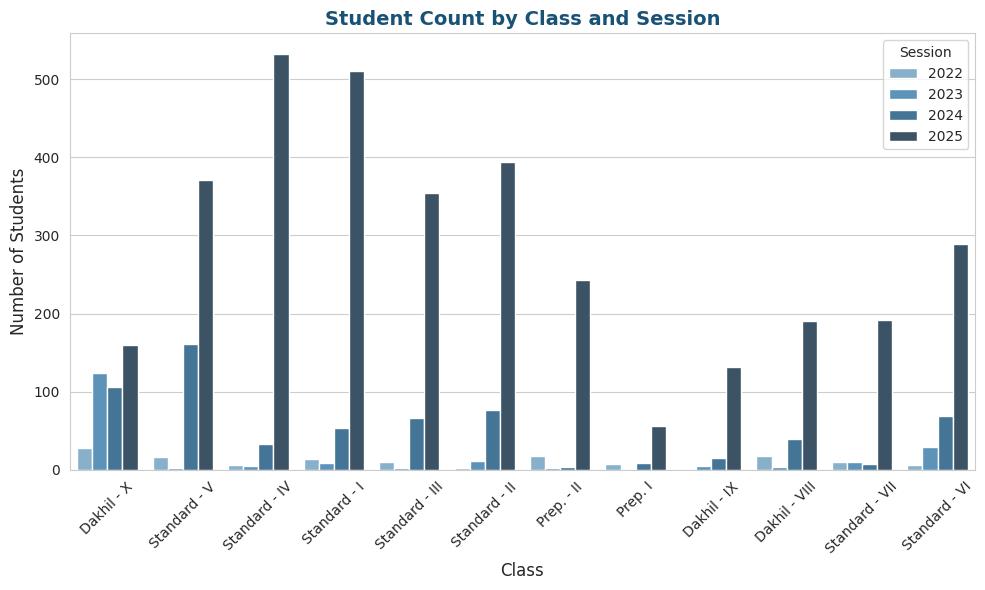
\includegraphics[width=\linewidth]{figures/fig2_class_session.png}
\caption{Record count by academic class and session. Coverage is strongly
non-uniform across grade levels and increases over the four sessions.}
\label{fig:classsession}
\end{figure}

Fig.~\ref{fig:groupdist} shows the distribution of academic group. Group
assignment is categorical rather than continuous and is unevenly populated,
so a model that predicts group from the printed text is solving a majority
class problem.

\begin{figure}[width=\linewidth,cols=1,pos=htbp]
\centering
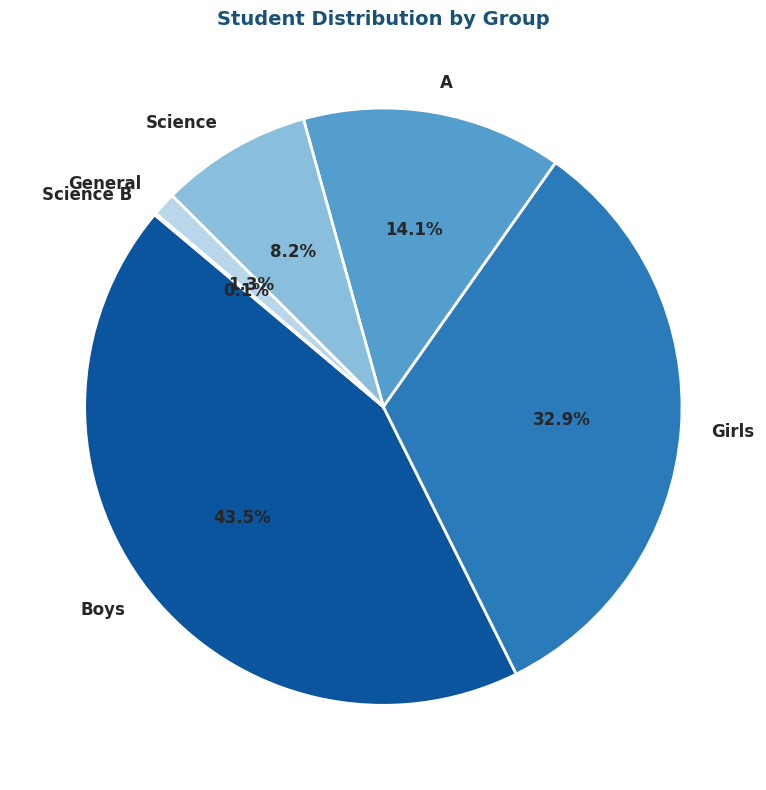
\includegraphics[width=\linewidth]{figures/fig3_group_pie.png}
\caption{Share of records by academic group. Group labels are short categorical
strings and are heavily skewed.}
\label{fig:groupdist}
\end{figure}

The lower band of each card lists registered subjects, and the vocabulary of
that band is the dominant source of lexical variety in the corpus.
Fig.~\ref{fig:subjfreq} ranks subjects by frequency. The head of the
distribution is short: a small set of compulsory subjects accounts for most
records, while the tail is long, containing optional and
specialisation-specific subjects that appear in only a few cards. For OCR
purposes this matters twice: frequent tokens dominate unweighted word error
rate, so a recogniser can score well while failing on exactly the rare
subjects that carry the most visual and lexical difficulty.

\begin{figure*}[width=\FullWidth,cols=1,pos=htbp]
\centering
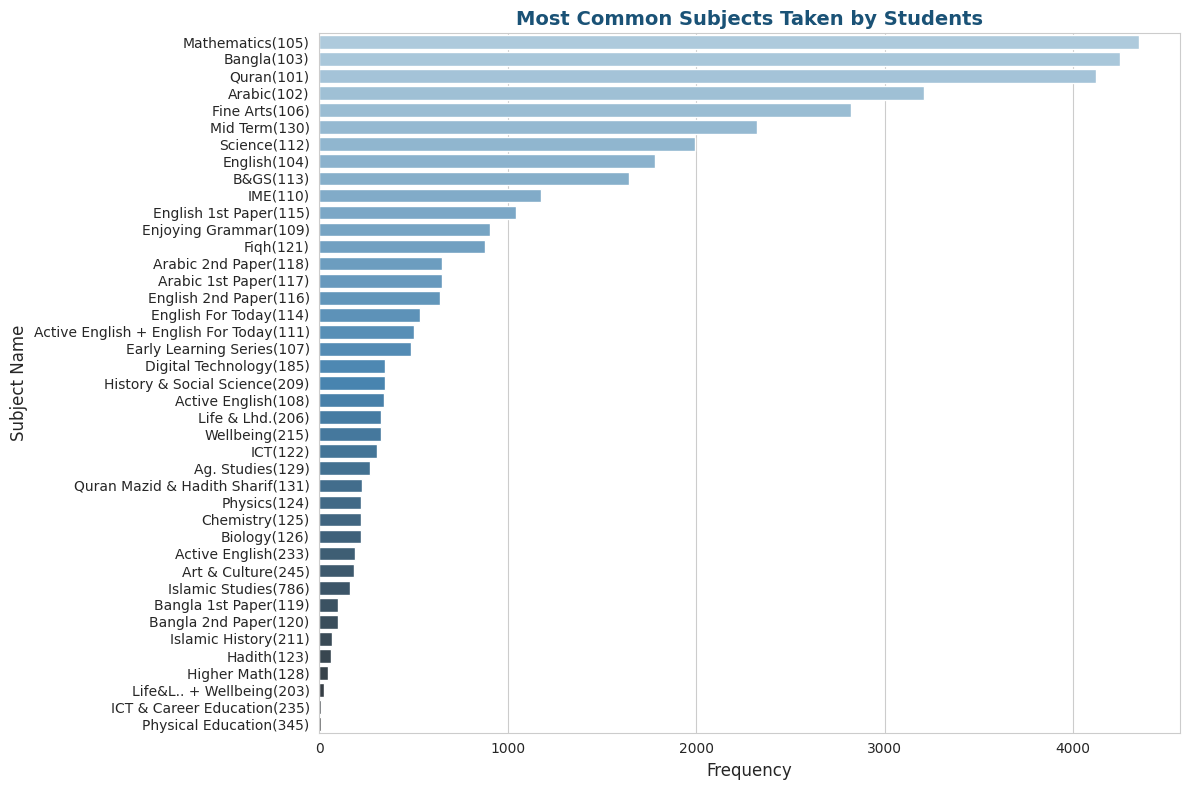
\includegraphics[width=\linewidth]{figures/fig4_subject_frequency.png}
\caption{Subject frequency across the corpus. The distribution has a short
head of compulsory subjects and a long tail of optional subjects, so
unweighted word error rate understates performance on the harder tail.}
\label{fig:subjfreq}
\end{figure*}

Finally, Fig.~\ref{fig:namelen} shows the distribution of name lengths for
students and their guardians. Names are the longest free-form strings on the
card, and the spread of lengths indicates the range of segmentation
difficulties a recogniser faces: short strings offer little context for
language modelling, while long strings accumulate error over more characters.
Because names in this corpus are synthetic substitutes of comparable length
(see Section~\ref{sec:ethics}), the length distribution is faithful to the
original even though the character content is not.

\begin{figure}[width=\linewidth,cols=1,pos=htbp]
\centering
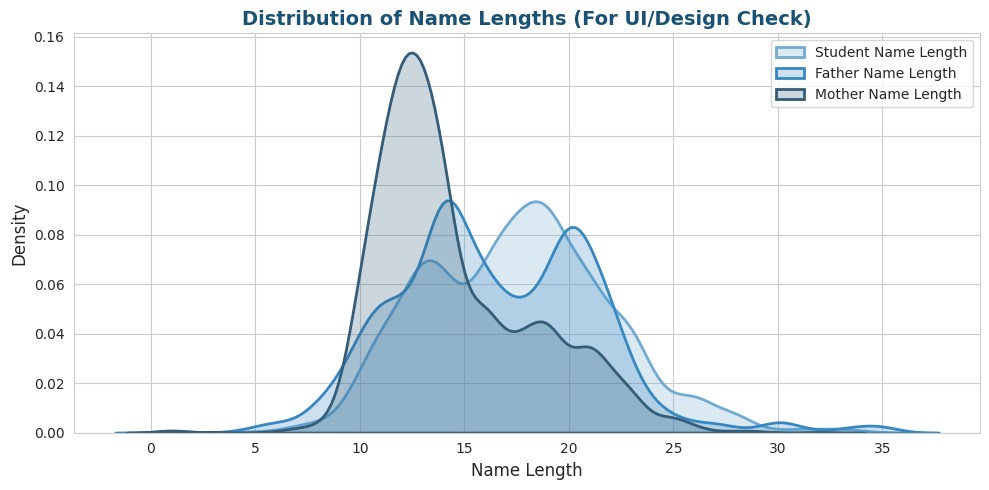
\includegraphics[width=\linewidth]{figures/fig5_name_length_kde.png}
\caption{Kernel density estimate of name lengths (characters) for students and
their guardians, showing the range of free-form string lengths present in the
corpus. Names are synthetic substitutes matched to the originals in length and
character class (Section~\ref{sec:ethics}), so the length distribution is
faithful to the original although the character content is not.}
\label{fig:namelen}
\end{figure}

%=================================================================
\section{Ground-truth annotation and quality assurance}
\label{sec:annotation}
%=================================================================

Ground truth was produced in two stages. First, the nine field values for each
card were read directly from the ERP database, guaranteeing that the
transcription matches what the issuing system believed it had printed. Second,
every record was inspected against its image to confirm that the rendered card
actually agrees with the database entry, and to catch records where the two had
drifted apart, for example after a late correction to a roll number. Records
failing this check were excluded rather than patched.

Two limitations of this procedure should be stated plainly. The verification
pass was performed by a single reviewer, so no inter-annotator agreement
statistic is available; the ground truth is authoritative with respect to the
issuing system but has not been independently replicated. And because
transcription is recorded per field rather than per character span, no
character-level bounding boxes are released. The fixed template makes field
regions approximately recoverable, but users requiring exact localisation
should derive and validate their own region definitions, and should measure
field-level accuracy as well as recognition accuracy, since a correctly
recognised string assigned to the wrong region is a failure mode that raw
character error rate does not expose.

%=================================================================
\section{Ethics, privacy and consent}
\label{sec:ethics}
%=================================================================

The corpus was compiled from records generated and retained by the institution
for official academic purposes. Release was authorised by the institution's
administration, which reviewed the procedure below before the data were
deposited. The design follows the data-minimisation and purpose-limitation
principles articulated in modern data protection regulation
\citep{gdpr2016}, applied here as a design reference for secondary research use
of administrative data.

Table~\ref{tab:privacy} lists the measures applied.

\begin{table}[width=\linewidth,cols=2,pos=htbp]
\rmfamily
\caption{Anonymisation and privacy measures applied before release.}
\label{tab:privacy}
\begin{tabular}{@{}P{0.28\linewidth}P{0.65\linewidth}@{}}
\toprule
\textbf{Measure} & \textbf{Implementation} \\
\midrule
Field selection
  & Only the nine fields required for OCR and layout research are retained;
    no academic results, grades or attendance data are included. \\
Content removal
  & Student photographs, signatures, contact numbers and any other personal
    identifiers present on the source cards are removed. \\
Identifier
randomisation
  & Names and institutional identifiers are replaced with synthetic
    substitutes matched to the original in token count, character class and
    script, so that length statistics and OCR difficulty are preserved. \\
Structure
preservation
  & Field order, template geometry, class, group, session and subject codes are
    left unaltered, since these carry the research value of the corpus. \\
Release control
  & Deposited on Mendeley Data under a citable DOI and version number so that
    the released state is fixed and auditable. \\
Permitted use
  & Academic and non-commercial research. Re-identification of any individual,
    or use for commercial or administrative decision-making about identifiable
    persons, is out of scope. \\
\bottomrule
\end{tabular}
\end{table}

One residual risk should not be understated. Randomisation protects the
identifiers themselves but not their context: the combination of class,
session, group and subject list is distinctive enough that, in principle, a
member of the original cohort could be narrowed down. The corpus should
therefore be treated as pseudonymised rather than anonymised data, and users
publishing derived results are advised not to report statistics at a
combination of fields fine enough to isolate an individual record. No such
attempt was made during preparation of this dataset.

%=================================================================
\section{Availability, versioning and reuse}
%=================================================================

The dataset is deposited on Mendeley Data as version~1 and is citable as
\citet{ashadzzaman2026}. Version numbers will be incremented for any
correction to the released files; the DOI resolves to the most recent version
while the version-specific URL remains resolvable in perpetuity. Users should
cite the version they used.

The corpus is intended for research on OCR and document understanding:
benchmarking recognition engines on production rather than synthetic
documents; training and evaluating key-information-extraction models for
fixed-schema administrative forms; studying layout analysis of form-like
documents; and developing tamper-detection methods that require authentic
reference material from a real issuing pipeline. Distribution follows the
findability and accessibility principles set out by \citet{wilkinson2016},
namely a persistent identifier, a public repository, and a documented schema.

%=================================================================
\section{Limitations}
%=================================================================

The following constraints bound what can legitimately be concluded from this
corpus.

\begin{itemize}[leftmargin=*,nosep,labelsep=6pt]
\item \textbf{Single institution, single system.} All records originate from
one school and one ERP configuration. Card templates elsewhere in the region
will differ in field inventory, nomenclature and typography; results obtained
here should not be assumed to transfer without re-evaluation.
\item \textbf{English text only.} Bangla, Arabic and English subject names
appear, but all personal names are Latin script. The corpus does not represent
Bangla or Arabic orthography and cannot support work on those scripts.
\item \textbf{Synthetic names.} Personal names were replaced. Length and
character-class distributions are preserved, but the corpus cannot be used to
study recognition of real Bangladeshi personal nomenclature, name matching, or
name-based entity resolution.
\item \textbf{No character-level ground truth.} Transcriptions are per field;
exact character bounding boxes are not released
(Section~\ref{sec:annotation}).
\item \textbf{Fixed acquisition.} All images are $800 \times 460$ pixels in a
single JPEG encoding. Performance at other resolutions, under recompression or
on physical scans is not characterised by this corpus.
\item \textbf{No photographs.} Faces were removed before release, so the corpus
is unsuitable for any biometric task.
\item \textbf{Class imbalance.} Coverage varies substantially across classes
and sessions (Fig.~\ref{fig:classsession}), and unweighted accuracy estimates
will be dominated by the largest groups.
\end{itemize}

%=================================================================
\section*{Acknowledgements}
%=================================================================

The author thanks the administration and management of Al Quran Academy,
Boalkhali, Chattogram, for authorising access to the examination archive and for
reviewing the anonymisation procedure, and the technical staff of the
NationalSchoolIntra platform for assistance in extracting the card records.

%=================================================================
\section*{Declaration of competing interest}
%=================================================================

The author declares no known competing financial interests or personal
relationships that could have influenced the work reported in this paper.

%=================================================================
\section*{Data availability}
%=================================================================

The EACS Dataset is publicly available on Mendeley Data at \dataseturl,
doi: \datasetdoiurl. Recommended citation:

\begingroup
\raggedright
Ashadzzaman, Baizid MD (2026), ``EACS Dataset: A Real-World Academic Admit
Card Dataset from Bangladeshi Educational Institutions for OCR and Document
Verification Research'', Mendeley Data, V1, doi: \datasetdoiurl.
\par
\endgroup

% To print the credit authorship contribution details
\printcredits

% ---- Bibliography -------------------------------------------------
\bibliographystyle{cas-model2-names}
\bibliography{eacs-refs}

\end{document}
